%!Mode:: "TeX:UTF-8"
\documentclass[a4paper,11pt,UTF8]{ctexart}

\usepackage{indentfirst} %缩进
\usepackage{xeCJK}    %使用系统字体
\usepackage{fancyhdr} %自定义页眉页脚
\pagestyle{plain}                   %不设置页眉页脚
\usepackage{amsmath, amsthm, amssymb, amsfonts} %数学公式
\usepackage[a4paper,left=3cm,right=3cm,top=3cm,bottom=3cm]{geometry}
%\usepackage[tmargin=1in,bmargin=1in,lmargin=1.25in,rmargin=1.25in]{geometry}.
\usepackage{booktabs} %插入表格
\usepackage[section]{placeins} %避免浮动
\usepackage{listings} %插入代码
\usepackage{ctex}     %中文宏包
\usepackage{bm}
\usepackage[svgnames, table]{xcolor} %彩色表格
\usepackage{algorithm}          %伪代码
\usepackage{algorithmicx}
\usepackage{algpseudocode}
\usepackage{algorithm,algpseudocode,float}
\usepackage{lipsum}
\usepackage{enumitem}           %调整列举环境
\usepackage{hyperref}
\hypersetup{
    colorlinks=true,
    linkcolor=blue,
    filecolor=blue,      
    urlcolor=blue,
    citecolor=cyan,
}
\usepackage{fontspec,xunicode}
\defaultfontfeatures{Mapping=tex-text} %如果没有它,会有一些 tex 特殊字符无法正常使用,比如连字符。

\usepackage{graphicx}
\graphicspath{{imgs/}}

%%%%%%%%%%%%%%%%%%%%%%%%%%%%%%%%%%%%%%%%%%%%%%%%%%%%%%%%%%%%%%%%
% 缩进及行间距
%%%%%%%%%%%%%%%%%%%%%%%%%%%%%%%%%%%%%%%%%%%%%%%%%%%%%%%%%%%%%%%%
\setlength{\parindent}{22pt} %重新定义缩进长度
\setlength{\baselineskip}{20pt}  %定义行间距
%\renewcommand{\baselinestretch}{1.1} %定义行间距

%%%%%%%%%%%%%%%%%%%%%%%%%%%%%%%%%%%%%%%%%%%%%%%%%%%%%%%%%%%%%%%%
% 列表设置
%%%%%%%%%%%%%%%%%%%%%%%%%%%%%%%%%%%%%%%%%%%%%%%%%%%%%%%%%%%%%%%%
\setenumerate{fullwidth,itemindent=\parindent,listparindent=\parindent,itemsep=0ex,partopsep=0pt,parsep=0ex}
\setenumerate[2]{label=\alph*),leftmargin=1.5em}  %二级item设置
\setitemize{itemindent=38pt,leftmargin=0pt,itemsep=-0.4ex,listparindent=26pt,partopsep=0pt,parsep=0.5ex,topsep=-0.25ex}
\setdescription{itemindent=38pt,leftmargin=0pt,itemsep=-0.4ex,listparindent=26pt,partopsep=0pt,parsep=0.5ex,topsep=-0.25ex}

%%%%%%%%%%%%%%%%%%%%%%%%%%%%%%%%%%%%%%%%%%%%%%%%%%%%%%%%%%%%%%%%
% 图的标题行间距设置
%%%%%%%%%%%%%%%%%%%%%%%%%%%%%%%%%%%%%%%%%%%%%%%%%%%%%%%%%%%%%%%%
\newcommand{\bottomcaption}{%
\setlength{\abovecaptionskip}{6pt}%
\setlength{\belowcaptionskip}{6pt}%
\caption}


%%%%%%%%%%%%%%%%%%%%%%%%%%%%%%%%%%%%%%%%%%%%%%%%%%%%%%%%%%%%%%%%
% 字体定义
%%%%%%%%%%%%%%%%%%%%%%%%%%%%%%%%%%%%%%%%%%%%%%%%%%%%%%%%%%%%%%%%
% \setmainfont{Times New Roman}  %默认英文字体.serif是有衬线字体sans serif无衬线字体
\setmonofont{Consolas}
\setCJKmainfont[ItalicFont={楷体}, BoldFont={黑体}]{宋体}%衬线字体 缺省中文字体为
\setCJKsansfont{黑体}
\punctstyle{hangmobanjiao}
%-----------------------xeCJK下设置中文字体------------------------------%
\setCJKfamilyfont{song}{SimSun}                             %宋体 song
\newcommand{\song}{\CJKfamily{song}}
\setCJKfamilyfont{fs}{FangSong}                      %仿宋  fs
\newcommand{\fs}{\CJKfamily{fs}}
\setCJKfamilyfont{ktgb}{KaiTi}                      %楷体2312 ktgb
\newcommand{\ktgb}{\CJKfamily{ktgb}}
\setCJKfamilyfont{yh}{Microsoft YaHei}                    %微软雅黑 yh
\newcommand{\yh}{\CJKfamily{yh}}
\setCJKfamilyfont{hei}{SimHei}                              %黑体  hei
\newcommand{\hei}{\CJKfamily{hei}}
\setCJKfamilyfont{hwxk}{STXingkai}                                %华文行楷  hwxk
\newcommand{\hwxk}{\CJKfamily{hwxk}}
%------------------------------设置字体大小------------------------%
\newcommand{\shiyanbaogao}{\fontsize{36pt}{\baselineskip}\selectfont}
\newcommand{\chuhao}{\fontsize{42pt}{\baselineskip}\selectfont}     %初号
\newcommand{\xiaochuhao}{\fontsize{36pt}{\baselineskip}\selectfont} %小初号
\newcommand{\yihao}{\fontsize{28pt}{\baselineskip}\selectfont}      %一号
\newcommand{\erhao}{\fontsize{21pt}{\baselineskip}\selectfont}      %二号
\newcommand{\xiaoerhao}{\fontsize{18pt}{\baselineskip}\selectfont}  %小二号
\newcommand{\sanhao}{\fontsize{15.75pt}{\baselineskip}\selectfont}  %三号
\newcommand{\sihao}{\fontsize{14pt}{\baselineskip}\selectfont}       %四号
\newcommand{\xiaosihao}{\fontsize{12pt}{\baselineskip}\selectfont}  %小四号
\newcommand{\wuhao}{\fontsize{10.5pt}{\baselineskip}\selectfont}    %五号
\newcommand{\xiaowuhao}{\fontsize{9pt}{\baselineskip}\selectfont}   %小五号
\newcommand{\liuhao}{\fontsize{7.875pt}{\baselineskip}\selectfont}  %六号
\newcommand{\qihao}{\fontsize{5.25pt}{\baselineskip}\selectfont}    %七号

%%%%%%%%%%%%%%%%%%%%%%%%%%%%%%%%%%%%%%%%%%%%%%%%%%%%%%%%%%%%%%%%
% 图题字体大小相同
%%%%%%%%%%%%%%%%%%%%%%%%%%%%%%%%%%%%%%%%%%%%%%%%%%%%%%%%%%%%%%%%
\usepackage{caption}
\captionsetup{font={footnotesize}}   % footnotesize = 9pt
\captionsetup[lstlisting]{font={footnotesize}}

%%%%%%%%%%%%%%%%%%%%%%%%%%%%%%%%%%%%%%%%%%%%%%%%%%%%%%%%%%%%%%%%
% 重定义枚举编号为 1),2)...
%%%%%%%%%%%%%%%%%%%%%%%%%%%%%%%%%%%%%%%%%%%%%%%%%%%%%%%%%%%%%%%%
\renewcommand{\labelenumi}{\theenumi)}


%%%%%%%%%%%%%%%%%%%%%%%%%%%%%%%%%%%%%%%%%%%%%%%%%%%%%%%%%%%%%%%%
% 重定义section标题
%%%%%%%%%%%%%%%%%%%%%%%%%%%%%%%%%%%%%%%%%%%%%%%%%%%%%%%%%%%%%%%%
\CTEXsetup[format={\sihao\CJKfamily{zhhei}\zihao{4}},number={\chinese{section}},name={,、~},aftername={},indent={0pt},beforeskip={6pt},afterskip={6pt},format+={\flushleft}]{section}
\CTEXsetup[format={\Large\bfseries\CJKfamily{zhkai}\zihao{4}},name={(,)},number={\chinese{subsection}},aftername={},indent={22pt},beforeskip={14pt},afterskip={2pt}]{subsection}
\CTEXsetup[number={\chinese{section}},name={附录, ~~ }]{appendix}



%%%%%%%%%%%%%%%%%%%%%%%%%%%%%%%%%%%%%%%%%%%%%%%%%%%%%%%%%%%%%%%%
% 标题名称中文化
%%%%%%%%%%%%%%%%%%%%%%%%%%%%%%%%%%%%%%%%%%%%%%%%%%%%%%%%%%%%%%%%
\renewcommand\figurename{\hei 图}
\renewcommand\tablename{\hei 表}
\renewcommand\lstlistingname{\hei 代码}
\renewcommand{\algorithmicrequire}{\textbf{输入:}}
\renewcommand{\algorithmicensure}{\textbf{输出:}}
\newtheorem{define}{定义}

%%%%%%%%%%%%%%%%%%%%%%%%%%%%%%%%%%%%%%%%%%%%%%%%%%%%%%%%%%%%%%%%
% 代码设置
%%%%%%%%%%%%%%%%%%%%%%%%%%%%%%%%%%%%%%%%%%%%%%%%%%%%%%%%%%%%%%%%
\lstset{
 columns=fixed,
 numbers=left,                                        % 在左侧显示行号
 numberstyle=\tiny\color{gray},                       % 设定行号格式
 frame=single,                                        % 单线背景边框
 breaklines=true,                                     % 设定LaTeX对过长的代码行进行自动换行
 keywordstyle=\color[RGB]{40,40,255},                 % 设定关键字颜色
 numberstyle=\footnotesize\color{darkgray},
 commentstyle=\it\color[RGB]{0,96,96},                % 设置代码注释的格式
 stringstyle=\rmfamily\slshape\color[RGB]{128,0,0},   % 设置字符串格式
 showstringspaces=false,                              % 不显示字符串中的空格
 language=java,                                        % 设置语言
 basicstyle=\linespread{1.0}\xiaowuhao\ttfamily,                      % 字体字号
 %lineskip=10pt,
 %baselinestretch=1,
}

%%%%%%%%%%%%%%%%%%%%%%%%%%%%%%%%%%%%%%%%%%%%%%%%%%%%%%%%%%%%%%%%
% 伪代码分页
%%%%%%%%%%%%%%%%%%%%%%%%%%%%%%%%%%%%%%%%%%%%%%%%%%%%%%%%%%%%%%%%
\makeatletter
\renewcommand{\ALG@name}{算法}
\newenvironment{breakablealgorithm}
  {% \begin{breakablealgorithm}
   \begin{center}
     \refstepcounter{algorithm}% New algorithm
     \hrule height.8pt depth0pt \kern2pt% \@fs@pre for \@fs@ruled
     \renewcommand{\caption}[2][\relax]{% Make a new \caption
       {\raggedright\textbf{\ALG@name~\thealgorithm} ##2\par}%
       \ifx\relax##1\relax % #1 is \relax
         \addcontentsline{loa}{algorithm}{\protect\numberline{\thealgorithm}##2}%
       \else % #1 is not \relax
         \addcontentsline{loa}{algorithm}{\protect\numberline{\thealgorithm}##1}%
       \fi
       \kern2pt\hrule\kern2pt
     }
  }{% \end{breakablealgorithm}
     \kern2pt\hrule\relax% \@fs@post for \@fs@ruled
   \end{center}
  }
\makeatother



\begin{document}
\xiaosihao\song

\begin{titlepage}
\center{\yihao{\hei{机器学习课程实验报告}}}
\vspace{6cm}
\center{\erhao{\ktgb{k-means聚类方法和混合高斯模型}}}
\vspace{4cm}

\begin{center}
\begin{large}
\begin{tabular}{rc}
\xiaoerhao{\hei{学\qquad 号}}& \hspace{1.7cm}\xiaoerhao{\hei{1180301007\hspace{1.7cm}}} \\
\cline{2-2}\\
\xiaoerhao{\hei{姓\qquad 名}}& \xiaoerhao{\hei{赵锦涛}}\\
\cline{2-2}\\
\xiaoerhao{\hei{实验时间}}& \xiaoerhao{\hei{2020年10月}}\\
\cline{2-2}
\end{tabular}
\end{large}
\end{center}
\vfill \hfill
\end{titlepage}
\clearpage


\setlength{\parskip}{6pt}  %定义段间距

\section{实验目的:}
实现一个k-means算法和混合高斯模型,并且用EM算法估计模型中的参数。
\section{实验要求:}
用高斯分布产生k个高斯分布的数据(不同均值和方差)(其中参数自己设定)。 \\
(1)用k-means聚类,测试效果; \\
(2)用混合高斯模型和你实现的EM算法估计参数,看看每次迭代后似然值变化情况,考察EM算法是否可以获得正确的结果(与你设定的结果比较)。 \\
应用:可以UCI上找一个简单问题数据,用你实现的GMM进行聚类。

\section{实验环境:}
Python 3.8, Windows 10
\section{实验原理:}
\subsection{k-means}
k-means 算法是一种基于划分的聚类算法,它以 k 为参数,把 n 个数据对象分成 k 个簇,使簇内具有较高的相似度,而簇间的相似度较低。 
k-means 算法是根据给定的 n 个数据对象的数据集,构建 k 个划分聚类的方法,每个划分聚类即为一个簇。该方法将数据划分为 n 个簇,每个簇至少有一个数据对象,每个数据对象必须属于而且只能属于一个簇。同时要满足同一簇中的数据对象相似度高,不同簇中的数据对象相似度较小。聚类相似度是利用各簇中对象的均值来进行计算的。
k-means 算法的处理流程如下。首先,随机地选择 k 个数据对象,每个数据对象代表一个簇中心,即选择 k 个初始中心;对剩余的每个对象,根据其与各簇中心的相似度(距离),将它赋给与其最相似的簇中心对应的簇;然后重新计算每个簇中所有对象的平均值,作为新的簇中心。
不断重复以上这个过程,直到准则函数收敛,也就是簇中心不发生明显的变化。通常采用均方差作为准则函数,即最小化每个点到最近簇中心的距离的平方和。k-means方法的复杂度为$O(mnk),其中m是样本维数,n是样本个数,k是类别个数$
\subsection{混合高斯模型与EM算法}
高斯混合模型假设数据中存在一定数量的高斯分布,并且每个分布代表一个簇,因此,高斯混合模型倾向于将属于同一分布的样本聚合为一类。
高斯混合模型可以理解为一个将事物分解为若干的基于高斯概率密度函数(正态分布曲线)形成的模型。多个高斯分布函数的线性组合,理论上GMM可以拟合出任意类型的分布。 \\
一种优雅的并且强大的寻找带有潜在变量的模型的最大似然解的方法被称为期望最大化算法,或者EM算法。给定一个高斯混合模型,目标是关于参数(均值、协方差、混合系数)最大化似然函数。算法流程如下:
\begin{itemize}
	\item 初始化均值$\mu_{k}$、协⽅差$\Sigma_{k}$和混合系数$\pi_{k}$,计算对数似然函数的初始值。
	\item E步骤。使⽤当前参数值计算“责任”。 $$
\gamma\left(z_{n k}\right)=\frac{\pi_{k} \mathcal{N}\left(\boldsymbol{x}_{n} \mid \boldsymbol{\mu}_{k}, \mathbf{\Sigma}_{k}\right)}{\sum_{j=1}^{K} \pi_{j} \mathcal{N}\left(\boldsymbol{x}_{n} \mid \boldsymbol{\mu}_{j}, \mathbf{\Sigma}_{j}\right)}
$$
	\item M步骤。使用当前的“责任”重新估计参数。 $$
\begin{aligned}
\boldsymbol{\mu}_{k}^{\text {new }} &=\frac{1}{N_{k}} \sum_{n=1}^{N} \gamma\left(z_{n k}\right) \mathbf{x}_{n} \\
\boldsymbol{\Sigma}_{k}^{\text {new }} &=\frac{1}{N_{k}} \sum_{n=1}^{N} \gamma\left(z_{n k}\right)\left(\mathbf{x}_{n}-\boldsymbol{\mu}_{k}^{\text {new }}\right)\left(\mathbf{x}_{n}-\boldsymbol{\mu}_{k}^{\text {new }}\right)^{\mathrm{T}} \\
\pi_{k}^{\text {new }} &=\frac{N_{k}}{N}
\end{aligned}
$$ \\
其中 $N_{k} = \sum_{n=1}^{N} \gamma(z_{nk})$
	\item 计算对数似然函数 $$
\ln p(\boldsymbol{X} \mid \boldsymbol{\mu}, \boldsymbol{\Sigma}, \boldsymbol{\pi})=\sum_{n=1}^{N} \ln \left\{\sum_{k=1}^{K} \pi_{k} \mathcal{N}\left(\boldsymbol{x}_{n} \mid \boldsymbol{\mu}_{k}, \boldsymbol{\Sigma}_{k}\right)\right\}
$$
\end{itemize}
检查参数或者对数似然函数的收敛性。如果没有满⾜收敛的准则,则返回第2步。
\section{代码实现}
本次实验共有5个文件,其名称和作用分别为:
\begin{itemize}
  \item \emph{datagen.py} \quad 生成训练数据
  \item \emph{kmeans.py} \quad k-means算法实现
  \item \emph{GMM\_EM.py} \quad 混合高斯模型实现与EM算法
  \item \emph{uci.py} \quad 对UCI数据集进行预处理
  \item \emph{uci\_gmm.py} \quad 对UCI数据集使用GMM模型EM算法进行聚类
\end{itemize}
在本次实验中,自主生成的数据样本共有两个维度,分为三个高斯分布,其均值分别为$[-2,2],[6.5,8],[10,-2]$,协方差矩阵均为$$
\begin{bmatrix}
	0.5 & 0 \\
	0 & 0.5 \\
\end{bmatrix}
$$
UCI数据集使用的是Iris数据集,具体信息请见\href{https://archive.ics.uci.edu/ml/datasets/Iris/}{Iris Data Set}
\section{实验结果与分析}
使用k-means算法对生成数据进行聚类,效果如图所示: \\
\begin{figure}[H]
  \centering
  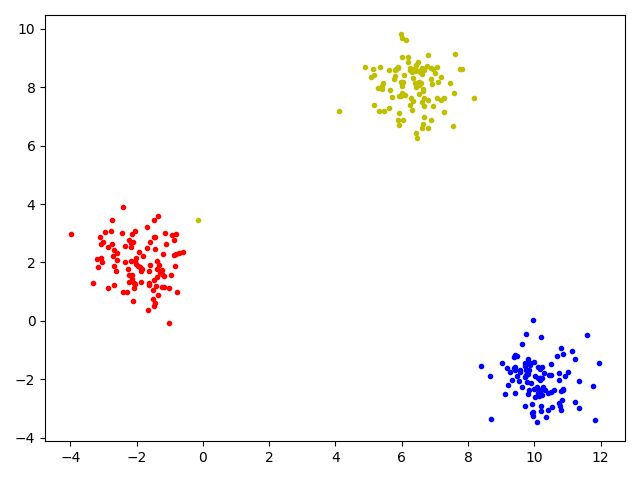
\includegraphics[width=0.6\textwidth]{kmeans.png}
  \bottomcaption{k-means}
\end{figure}
使用GMM模型EM算法对生成数据进行聚类,效果如图所示:\\
\begin{figure}[H]
  \centering
  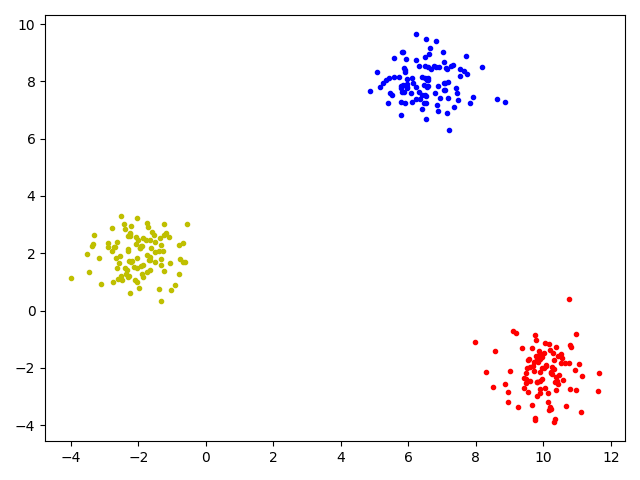
\includegraphics[width=0.6\textwidth]{gmm.png}
  \bottomcaption{GMM}
\end{figure}
使用EM算法对UCI数据进行聚类,结果如图:\\
\begin{figure}[H]
  \centering
  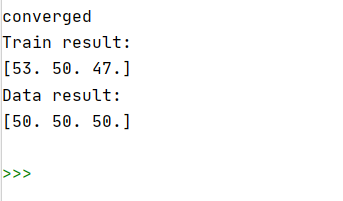
\includegraphics[width=0.6\textwidth]{uci.png}
  \bottomcaption{Iris}
\end{figure}
从实验结果可以看出,k-means算法和EM算法均能对数据进行较好的聚类。在实验中发现,GMM模型对初始点的选择有要求,如果初始点选择地不好,则聚类结果可能会很差。一般的做法是使用k-means算法计算得到中心点,然后用该中心点来初始化GMM模型的均值。
\begin{thebibliography}{99} 
\bibitem{ref1}Bishop C M. Pattern recognition and machine learning[M]. springer, 2006.
\end{thebibliography}



\end{document}
